\documentclass[12pt,letterpaper]{article}
\usepackage{fullpage}
\usepackage[top=2cm, bottom=4.5cm, left=2.5cm, right=2.5cm]{geometry}
\usepackage{amsmath,amsthm,amsfonts,amssymb,amscd}
\usepackage{lastpage}
\usepackage{enumerate}
\usepackage{fancyhdr}
\usepackage{mathrsfs}
\usepackage{xcolor}
\usepackage{fancyvrb}
\usepackage{graphicx}
\usepackage{listings}
\usepackage{float}
\usepackage{hyperref}
\usepackage{tikz}
\usepackage{relsize}
\usepackage{fancyvrb}
\usepackage{multirow}
\usepackage{booktabs}
\usepackage{import}
\usetikzlibrary{shapes.geometric,fit}

\hypersetup{%
  colorlinks=true,
  linkcolor=blue,
  linkbordercolor={0 0 1}
}

\setlength{\parindent}{0.0in}
\setlength{\parskip}{0.05in}

\theoremstyle{definition}
\newtheorem*{statement}{Statement}
\newtheorem*{claim}{Claim}
\newtheorem*{theorem}{Theorem}
\newtheorem*{lemma}{Lemma}

\newcommand{\contra}{\Rightarrow\!\Leftarrow}
\newcommand{\R}{\mathbb{R}}
\newcommand{\F}{\mathbb{F}}
\newcommand{\Z}{\mathbb{Z}}
\newcommand{\Zeq}{\mathbb{Z}_{\geq 0}}
\newcommand{\Zg}{\mathbb{Z}_{>0}}
\newcommand{\Req}{\mathbb{R}_{\geq 0}}
\newcommand{\Rg}{\mathbb{R}_{>0}}
\newcommand{\N}{\mathbb{N}}
\newcommand{\Q}{\mathbb{Q}}
\newcommand{\C}{\mathbb{C}}
\DeclareMathOperator{\Cov}{Cov}
\DeclareMathOperator{\Var}{Var}

\newcommand{\incfig}[1] {%
    \import{./figures/}{#1.pdf_tex}
}

\graphicspath{ {./figures/} }

\title{ECON 3412 HW 7}
\author{David Chen, dc3451}

\begin{document}

\maketitle

\section*{Problem 1}
\subsection*{a}

We reproduce 1-3 as follows:
\begin{Verbatim}[fontsize=\small]
> ajr <- read_dta("./AJR2001.dta")

> ajr.ols <- lm(loggdp ~ risk, data = ajr)
> ajr.rfreg <- lm(risk ~ logmort0, data = ajr)
> ajr.ivreg <- ivreg(loggdp ~ risk | logmort0, data = ajr)
\end{Verbatim}
which respectively give us the ordinary least squares, the reduced form, and the instrument regression.

Checking the coefficients (with homoskedastic errors, since this is what the authors used):
\begin{Verbatim}[fontsize=\small]
> coeftest(ajr.ols)

t test of coefficients:

            Estimate Std. Error t value  Pr(>|t|)
(Intercept) 4.687415   0.417441 11.2289 < 2.2e-16 ***
risk        0.516187   0.062519  8.2565 1.421e-11 ***
---
Signif. codes:  0 ‘***’ 0.001 ‘**’ 0.01 ‘*’ 0.05 ‘.’ 0.1 ‘ ’ 1

> coeftest(ajr.rfreg)

t test of coefficients:

            Estimate Std. Error t value  Pr(>|t|)
(Intercept)  9.36589    0.61059 15.3390 < 2.2e-16 ***
logmort0    -0.61329    0.12694 -4.8313 9.273e-06 ***
---
Signif. codes:  0 ‘***’ 0.001 ‘**’ 0.01 ‘*’ 0.05 ‘.’ 0.1 ‘ ’ 1

> coeftest(ajr.ivreg)

t test of coefficients:

            Estimate Std. Error t value  Pr(>|t|)
(Intercept)  1.99430    1.02403  1.9475   0.05601 .
risk         0.92949    0.15609  5.9548 1.327e-07 ***
---
Signif. codes:  0 ‘***’ 0.001 ‘**’ 0.01 ‘*’ 0.05 ‘.’ 0.1 ‘ ’ 1
\end{Verbatim}

The coefficient on $risk$ varies from the paper's by $0.01$ ($0.93$ in this regression, but $0.94$ in the given one).

\subsection*{b}

Homoskedastic errors are given above, and match the given standard errors, so they used homoskedastic errors. Heteroskedastic errors are calculated below:
\begin{Verbatim}[fontsize=\small]
> coeftest(ajr.ols, vcovCL)

t test of coefficients:

            Estimate Std. Error t value  Pr(>|t|)
(Intercept) 4.687415   0.324474  14.446 < 2.2e-16 ***
risk        0.516187   0.051101  10.101 1.009e-14 ***
---
Signif. codes:  0 ‘***’ 0.001 ‘**’ 0.01 ‘*’ 0.05 ‘.’ 0.1 ‘ ’ 1

> coeftest(ajr.rfreg, vcovCL)

t test of coefficients:

            Estimate Std. Error t value  Pr(>|t|)
(Intercept)  9.36589    0.70841 13.2209 < 2.2e-16 ***
logmort0    -0.61329    0.15178 -4.0405 0.0001495 ***
---
Signif. codes:  0 ‘***’ 0.001 ‘**’ 0.01 ‘*’ 0.05 ‘.’ 0.1 ‘ ’ 1

> coeftest(ajr.ivreg, vcovCL)

t test of coefficients:

            Estimate Std. Error t value  Pr(>|t|)
(Intercept)  1.99430    1.14396  1.7433   0.08623 .
risk         0.92949    0.17143  5.4219 1.029e-06 ***
---
Signif. codes:  0 ‘***’ 0.001 ‘**’ 0.01 ‘*’ 0.05 ‘.’ 0.1 ‘ ’ 1
\end{Verbatim}

\subsection*{c}

We can calculate this by $\frac{\Cov(loggdp, logmort0)}{\Cov(risk, logmort0)} = \frac{-0.894}{-0.962} = 0.929$, so the same as above. Alternatively, we can regress $loggdp$ in $logmort0$ and divide by the coefficient on the reduce form regression, which comes out to $\frac{-0.57}{-0.613} = 0.929$ so we get the same estimate in every case here.
\begin{Verbatim}[fontsize=\small]
> lm(loggdp ~ logmort0, data = ajr)

Call:
lm(formula = loggdp ~ logmort0, data = ajr)

Coefficients:
(Intercept)     logmort0
      10.70        -0.57
\end{Verbatim}

\subsection*{d}

We just do this manually (discard the standard errors due to the double regression, so no heteroskedastic errors are computed).
\begin{Verbatim}[fontsize=\small]
> lm(loggdp ~ predict(ajr.rfreg), data = ajr)

Call:
lm(formula = loggdp ~ predict(ajr.rfreg), data = ajr)

Coefficients:
       (Intercept)  predict(ajr.rfreg)
            1.9943              0.9295

\end{Verbatim}
so we get the same regression as the earlier ones.

\subsection*{e}

Here, we regress on both $risk$ and the residuals of the reduced form as a control (I don't know how \textit{morally} different this is from standard TSLS, but we are not regressing on the predicted values of $risk$):
\begin{Verbatim}[fontsize=\small]
> coeftest(lm(loggdp ~ risk + ajr.rfreg$residuals, data = ajr), vcovCL)

t test of coefficients:

                     Estimate Std. Error t value  Pr(>|t|)
(Intercept)          1.994296   0.562095  3.5480 0.0007536 ***
risk                 0.929490   0.088528 10.4994 2.674e-15 ***
ajr.rfreg$residuals -0.568900   0.123449 -4.6084 2.121e-05 ***
---
Signif. codes:  0 ‘***’ 0.001 ‘**’ 0.01 ‘*’ 0.05 ‘.’ 0.1 ‘ ’ 1
\end{Verbatim}
so we get the same TSLS estimator of $0.929$ as earlier.

\subsection*{f}

\begin{Verbatim}[fontsize=\small]
> ajr.olsnew <- lm(loggdp ~ risk + africa + latitude, data = ajr)
> coeftest(ajr.olsnew, vcovCL)

t test of coefficients:

            Estimate Std. Error t value  Pr(>|t|)
(Intercept)  5.65223    0.38398 14.7202 < 2.2e-16 ***
risk         0.37652    0.06556  5.7432 3.284e-07 ***
africa      -0.72327    0.16945 -4.2682 7.114e-05 ***
latitude     1.38246    0.63496  2.1773   0.03341 *
---
Signif. codes:  0 ‘***’ 0.001 ‘**’ 0.01 ‘*’ 0.05 ‘.’ 0.1 ‘ ’ 1
\end{Verbatim}
Ordinary least squares gets us that $africa$ plays a statistically significant part in the regression with $p = 7.114e-05$ and $latitude$ as well at $p = 3.34e-02$, and since the coefficients are significantly nonzero, the regression does suggest that $latitude$ and $africa$ are predictive of the level of GDP.

\subsection*{g}

\begin{Verbatim}[fontsize=\small]
> ajr.ivregnew <- ivreg(loggdp ~ risk + africa + latitude |
+                         logmort0 + africa + latitude, data = ajr)
+ coeftest(ajr.ivregnew, vcovCL)
+
t test of coefficients:

             Estimate Std. Error t value Pr(>|t|)
(Intercept)  2.995070   1.756874  1.7048 0.093410 .
risk         0.799968   0.274386  2.9155 0.004987 **
africa      -0.347926   0.332082 -1.0477 0.298974
latitude    -0.055311   1.128031 -0.0490 0.961056
---
Signif. codes:  0 ‘***’ 0.001 ‘**’ 0.01 ‘*’ 0.05 ‘.’ 0.1 ‘ ’ 1
\end{Verbatim}
$latitude$ and $africa$ are no longer significantly different from $0$ in this regression, as opposed to earlier when they were. In this case, the regression does not suggest that $latitude$ and $africa$ are predictive of the level of GDP.

\subsection*{h}

We generated the variable with \verb|ajr$mort0 <- exp(ajr$logmort0)| and regress:
\begin{Verbatim}[fontsize=\small]
> ajr.rfregexp <- lm(risk ~ mort0, data = ajr)
> coeftest(ajr.rfregexp, vcovCL)

t test of coefficients:

               Estimate  Std. Error t value Pr(>|t|)
(Intercept)  6.70941894  0.20104139  33.373   <2e-16 ***
mort0       -0.00078616  0.00029666  -2.650   0.0102 *
---
Signif. codes:  0 ‘***’ 0.001 ‘**’ 0.01 ‘*’ 0.05 ‘.’ 0.1 ‘ ’ 1

\end{Verbatim}
we can see that the $t$-statistic in this regression is much lower (in magnitude) than the earlier reduced form with $logmort0$ (earlier it was $t = -4.045$ in the heteroskedastic regression, and $t = -4.83$ in the homoskedastic regression). However, it still is significant $p = 0.01$, even if the fit is worse (also $R^{2}$ decreased from $0.27$ to $0.064$). This worse fit is one reason that they used the log regression since you don't want weak instruments. Further, if we carry out the TSLS with $mort0$ instead of its logarithm, we get
\begin{Verbatim}[fontsize=\small]
> ajr.ivregexp <- ivreg(loggdp ~ risk | mort0, data = ajr)
> coeftest(ajr.ivregexp, vcovCL)

t test of coefficients:

            Estimate Std. Error t value Pr(>|t|)
(Intercept)  0.48869    3.25608  0.1501  0.88118
risk         1.16055    0.49595  2.3401  0.02251 *
---
Signif. codes:  0 ‘***’ 0.001 ‘**’ 0.01 ‘*’ 0.05 ‘.’ 0.1 ‘ ’ 1
\end{Verbatim}
which has the coefficient of $risk$ at a much higher $p$ than before.

\subsection*{i}

\begin{Verbatim}[fontsize=\small]
> ajr.rfregquad <- lm(risk ~ logmort0 + I(logmort0^2), data = ajr)
> coeftest(ajr.rfregquad, vcovCL)

t test of coefficients:

               Estimate Std. Error t value  Pr(>|t|)
(Intercept)   13.948594   1.618271  8.6194 3.808e-12 ***
logmort0      -2.645684   0.737166 -3.5890 0.0006622 ***
I(logmort0^2)  0.210114   0.081681  2.5724 0.0125508 *
---
Signif. codes:  0 ‘***’ 0.001 ‘**’ 0.01 ‘*’ 0.05 ‘.’ 0.1 ‘ ’ 1
\end{Verbatim}

We see that the relationship between $risk$ and $logmort0$ is significantly nonlinear since the coefficient of $logmort0^{2}$ is significantly nonzero ($p = 0.0125$). Then, the instrument regression becomes
\begin{Verbatim}[fontsize=\small]
> ajr.ivregquad <- ivreg(loggdp ~ risk | logmort0 + I(logmort0^2), data = ajr)
> coeftest(ajr.ivregquad, vcovCL)

t test of coefficients:

            Estimate Std. Error t value  Pr(>|t|)
(Intercept) 3.018849   0.676666  4.4614 3.498e-05 ***
risk        0.772255   0.099313  7.7760 9.687e-11 ***
---
Signif. codes:  0 ‘***’ 0.001 ‘**’ 0.01 ‘*’ 0.05 ‘.’ 0.1 ‘ ’ 1
\end{Verbatim}
which sees the coefficient on risk remain highly statistically significant $p = 9.687e-11$, but also lower in magnitude and of the same sign: $0.929$ to $0.772$. Thus, an exogenous unit change in the risk predicts a change of $77\%$ in the GDP / capita.

\subsection*{j}

\begin{Verbatim}[fontsize=\small]
> linearHypothesis(ajr.rfregquad, c("logmort0 = 0", "I(logmort0^2) = 0"),
+ vcov = vcovHC(ajr.rfregquad, "HC1"))
Linear hypothesis test

Hypothesis:
logmort0 = 0
I(logmort0^2) = 0

Model 1: restricted model
Model 2: risk ~ logmort0 + I(logmort0^2)

Note: Coefficient covariance matrix supplied.

  Res.Df Df      F   Pr(>F)
1     63
2     61  2 22.803 4.03e-08 ***
---
Signif. codes:  0 ‘***’ 0.001 ‘**’ 0.01 ‘*’ 0.05 ‘.’ 0.1 ‘ ’ 1
\end{Verbatim}
so $F > 10$ and we have that the instruments are strong.

\subsection*{k}

\begin{Verbatim}[fontsize=\small]
> ajr.Jtest <- lm(ajr.ivregquad$residuals ~ logmort0 + I(logmort0^2), data = ajr)
+ linearHypothesis(ajr.Jtest, c("logmort0 = 0", "I(logmort0^2) = 0"),
+                  vcov = vcovHC(ajr.Jtest, "HC1"))
+
Linear hypothesis test

Hypothesis:
logmort0 = 0
I(logmort0^2) = 0

Model 1: restricted model
Model 2: ajr.ivregquad$residuals ~ logmort0 + I(logmort0^2)

Note: Coefficient covariance matrix supplied.

  Res.Df Df     F Pr(>F)
1     63
2     61  2 1.354 0.2659
\end{Verbatim}
so $J = 2 \cdot 1.354 = 2.708$, and since it is $\chi^{2}$ distributed with $2- 1 = 1$ degree of freedom, and $pchisq(2.708, df=1) = 0.9001539$ so it is significant at $p = 0.10$. In particular, we fail to reject the null hypothesis (since usually we use $p = 0.05$) so this means that the instruments are exogenous and thus uncorrelated with the error in the TSLS: $\Cov(logmort0, u) = \Cov(logmort0^{2}, u) = 0$.

\section*{Problem 2}
\subsection*{a}

Transactions under the tax cut are red, transactions not under the tax cut are blue, the treatment group is green (same as red in the post tax cut phase), and the control is black. The $x$-axis is month (in given numerical format, not sure if STATA atomically converts it). $y$-axis is log of the amount of transactions (discard the axis labels).
\begin{Verbatim}[fontsize=\small]
bkh <- read_dta("./BKHousing.dta")
bkh$logBinCount <- log(bkh$BinCount)
bkh$Treatment <- bkh$UBound5K <= 175000
bkh$PostCut <- bkh$Month >= 584 & bkh$Month <= 599
bkh$HasCut <- bkh$Treatment & bkh$PostCut

bkh.MonthCut <- c()
bkh.MonthNoCut <- c()
bkh.Treatment <- c()
bkh.Control <- c()
for (month in unique(bkh$Month)) {
  if (length(bkh[bkh$Month == month & bkh$HasCut == 1,]$logBinCount) > 0) {
    cut <- mean(bkh[bkh$Month == month & bkh$HasCut == 1,]$logBinCount)
    bkh.MonthCut <- append(bkh.MonthCut, cut)
  }
  nocut <- mean(bkh[bkh$Month == month & bkh$HasCut == 0,]$logBinCount)
  bkh.MonthNoCut <- append(bkh.MonthNoCut, nocut)

  treat <- mean(bkh[bkh$Month == month & bkh$Treatment == 1,]$logBinCount)
  bkh.Treatment <- append(bkh.Treatment, treat)
  cont <- mean(bkh[bkh$Month == month & bkh$Treatment == 0,]$logBinCount)
  bkh.Control <- append(bkh.Control, cont)
}

ggplot() + geom_line(aes(x = unique(bkh$Month), y = bkh.MonthNoCut), color = "blue") +
  geom_point(aes(x = unique(bkh$Month), y = bkh.MonthNoCut), color = "blue") +
  geom_line(aes(x = unique(bkh$Month), y = bkh.Treatment), color="green") +
  geom_point(aes(x = unique(bkh$Month), y = bkh.Treatment), color = "green") +
  geom_line(aes(x = unique(bkh$Month), y = bkh.Control), color = "black") +
  geom_point(aes(x = unique(bkh$Month), y = bkh.Control), color = "black") +
  geom_line(aes(x = 584:599, y = bkh.MonthCut), color="red") +
  geom_point(aes(x = 584:599, y = bkh.MonthCut), color = "red")
\end{Verbatim}

\begin{figure}[H]
  \begin{center}
    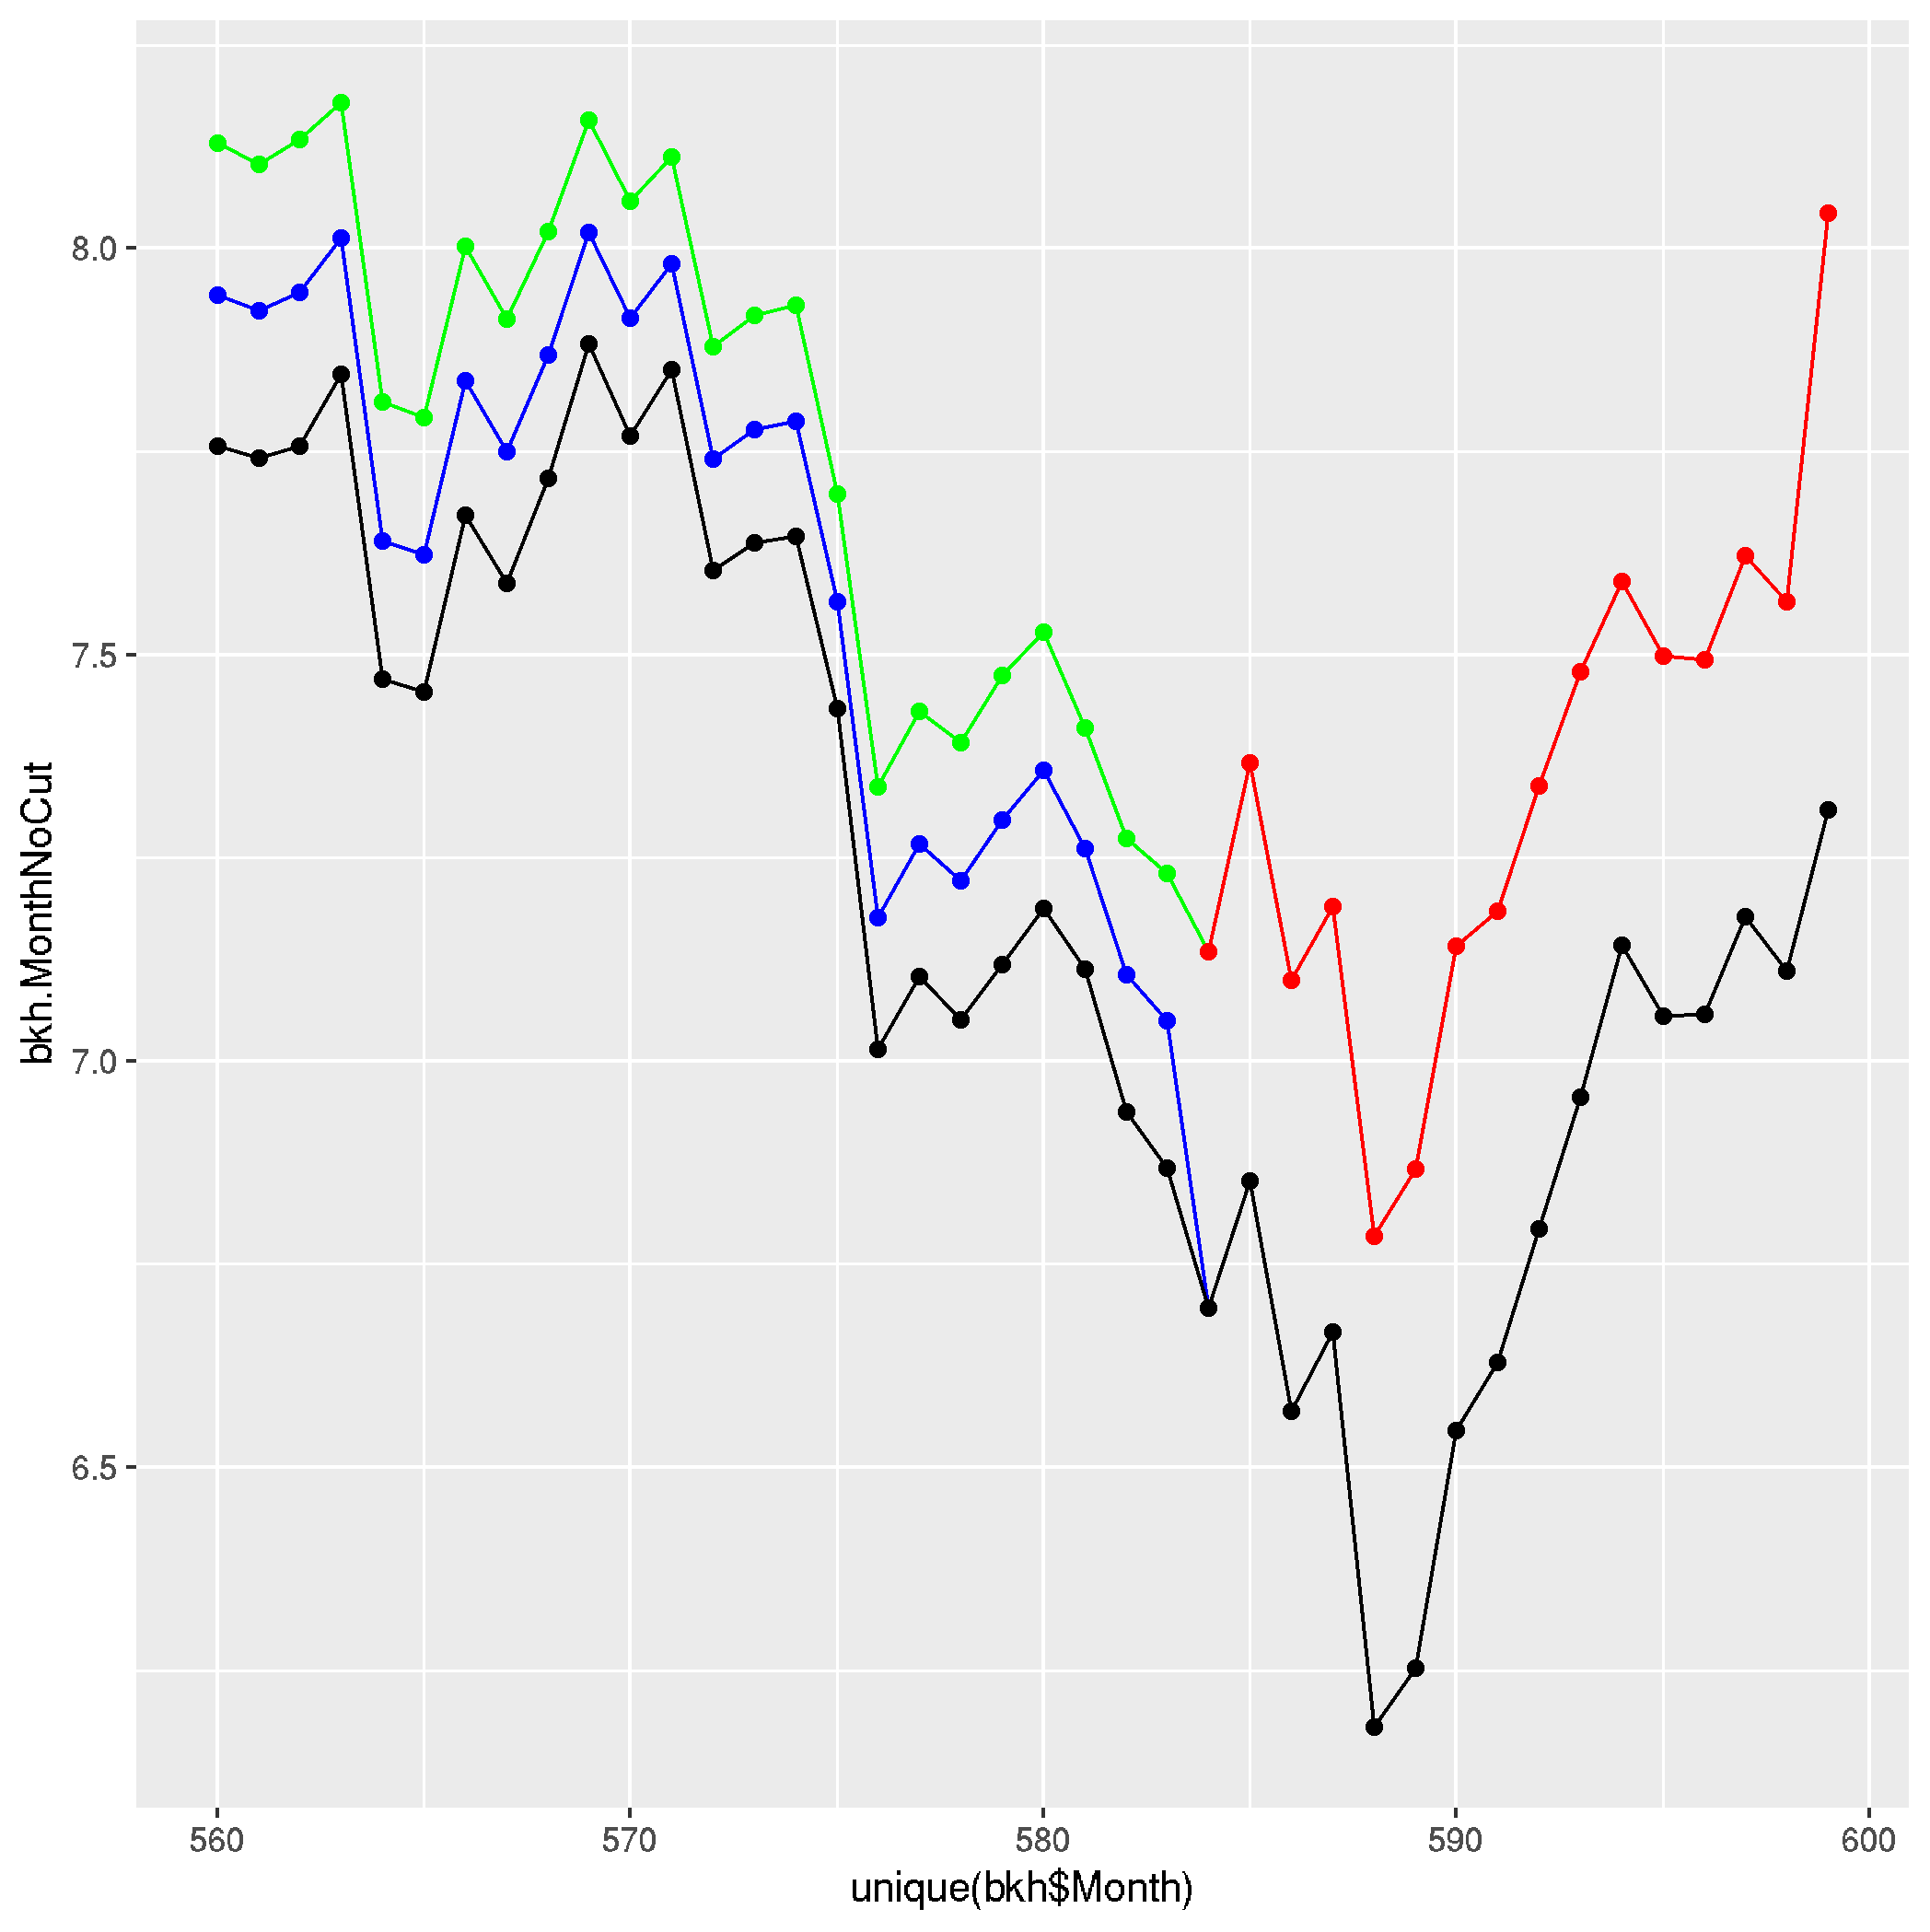
\includegraphics[width=10cm]{2a.png}
  \end{center}
\end{figure}

\subsection*{b}

\begin{Verbatim}[fontsize=\small]
> mean(bkh[bkh$Treatment & !bkh$PostCut,]$logBinCount)
[1] 7.788033
> mean(bkh[!bkh$Treatment & !bkh$PostCut,]$logBinCount)
[1] 7.467547
> mean(bkh[!bkh$Treatment & bkh$PostCut,]$logBinCount)
[1] 6.812198
> mean(bkh[bkh$Treatment & bkh$PostCut,]$logBinCount)
[1] 7.337447
\end{Verbatim}

\begin{table}[H]
  \centering
  \begin{tabular}{lll|l}
    \toprule
    & Treatment & Control & Difference \\
    \midrule
    Pre-tax cut & 7.788 & 7.467 & -0.321 \\
    Post-tax cut & 7.337 & 6.812 & -0.525 \\
    \midrule
    Difference & -0.451 & -0.655  & 0.204 \\
    \bottomrule
  \end{tabular}
\end{table}

\subsection*{c}

\begin{Verbatim}[fontsize=\small]
> bkh.dd <- plm(logBinCount ~ HasCut, data = bkh, index = c("UBound5K", "Month"),
+               model = "within", effect = "twoways")
+ coef_test(bkh.dd, vcov = "CR1S", cluster = bkh$UBound5K)
       Coef. Estimate     SE t-stat d.f. p-val (Satt) Sig.
1 HasCutTRUE    0.205 0.0403   5.09   18       <0.001  ***
\end{Verbatim}

The estimated difference-in-differences coefficient is statistically significant (that is, against the null that it is zero) at $p < 0.001$. The magnitude of the coefficient is that the difference between and after the tax cut in the logarithm of the amount of transactions in the group that received the tax cut is greater by $0.205$ compared to those that did not receive a tax cut; thus, this regression predicts that the tax cut prevented $20\%$ of transactions being lost in the price bins receiving the cut compared to the counterfactual where there was no cut at all.

\subsection*{d}

\begin{Verbatim}[fontsize=\small]
> bkh$Value <- bkh$UBound5K - 2500
+ bkh.ddint <- plm(logBinCount ~ HasCut + I(HasCut * Value), data = bkh,
+                  index = c("UBound5K", "Month"),
+                  model = "within", effect = "twoways")
+ coef_test(bkh.ddint, vcov = "CR1S", cluster = bkh$UBound5K)
+
              Coef.  Estimate       SE t-stat d.f. p-val (Satt) Sig.
1        HasCutTRUE  1.33e+00 1.76e-01   7.57 4.81      < 0.001  ***
2 I(HasCut * Value) -7.50e-06 1.11e-06  -6.73 4.77      0.00132   **
\end{Verbatim}

The interaction between the two variables is small (on the order of $10^{-6}$), but significantly nonzero. However, since the value is in the hundreds of thousands, the effect is relatively large. More specifically, in the treatment group, an movement from one price bin to the next, on average (the same as a $5K$ increase in the value) results in a change of $-7.50e-06 \cdot 5000 = -0.0375$, so we have that going up in value by $\$5000$ makes the percent of transactions that were stopped from being lost decreases by $3.65\%$. That is, the policy is less effective in higher price bins.

\subsection*{e}

\begin{Verbatim}[fontsize=\small]
> bkh$MonthInt <- bkh$HasCut * bkh$Month
+ bkh.ddtime <- plm(logBinCount ~ HasCut + MonthInt, data = bkh, index = c("UBound5K", "Month"),
+                  model = "within", effect = "twoways")
+ coef_test(bkh.ddtime, vcov = "CR1S", cluster = bkh$UBound5K)
>        Coef.  Estimate      SE t-stat d.f. p-val (Satt) Sig.
1 HasCutTRUE  0.419360 1.49669  0.280   18        0.783
2   MonthInt -0.000363 0.00249 -0.146   18        0.886
\end{Verbatim}
so we can see that there is no significant interaction with time here. The interpretation is that among the treated, the model predicts that there is no difference between different time periods after the implementation of the policy in terms of how effective it was compared to the earlier counterfactual.

\subsection*{f}

One problem here is that we might consider the control to be different from the treatment group. We found earlier that the higher the value of the price bin, the less effective the policy, so the control group might be less affected by the policy than the treatment group, since the control is entirely bins that are higher than the treatment group. This would bias the regression; a lot of other threats aren't applicable here, i.e. experimenter bias or attrition. We also don't know anything about inclusion/exclusion failures of this policy (though I'd guess that its low on both sides) so attrition errors are possible as well.

All this being said, we still do see that there is a significant saving of real estate transactions from the policy, so if the goal is to stimulate spending after a COVID recession, then this policy is still an option.

\end{document}
% LocalWords:  NetID fancyplain LocalWords colorlinks linkcolor linkbordercolor
